\chapter{Induction électromagnétique}


\paragraph{Objectif}

\begin{enumerate}
  \item L'étudiant connaîtra le concept de flux magnétique.
  \item L'étudiant connaîtra la loi de Lenz-Faraday.
\end{enumerate}


\section{Flux magnétique}

\marginnote{
  Lafrance \S 10.2
}

Le flux magnétique $\Phi_B$ est une mesure du nombre de lignes de champ qui
traversent une surface. Pour aider à comprendre, il est utile de faire une
analogie avec un fluide.


\begin{diapobox}

Classez les situations suivantes en ordre croissant de la quantité de liquide
qui passe à travers le cadre.

\begin{center}
  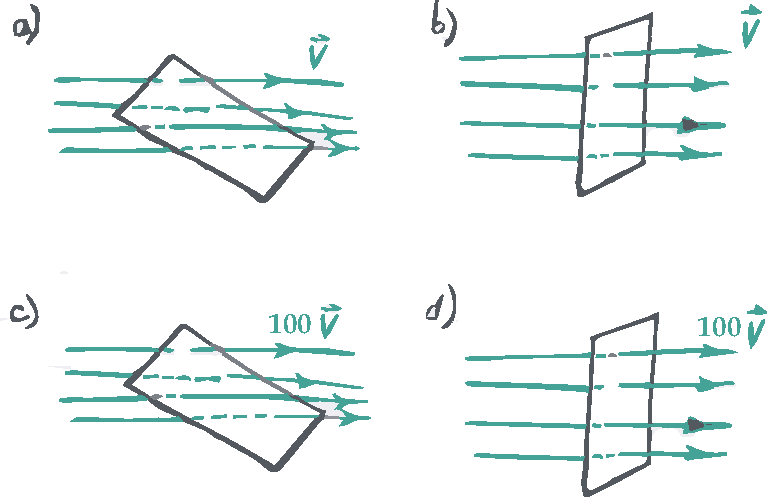
\includegraphics[scale=0.8]{10-induction-electromagnetique/figures/flux.pdf}
\end{center}

\end{diapobox}


\subsection*{Définition du flux magnétique}

On veut donc que le flux soit proportionnel à la composante du champ magnétique
perpendiculaire à la surface et à l'aire. Donc
$$\Phi_B = BA\cos\theta$$
Si on définit $\vec{A}$ comme un vecteur dont la longueur est l'aire de la
surface et qui est perpendiculaire à la surface, alors
$$\Phi_B = \vB \cdot \vec{A}$$

Si le champ magnétique n'est pas uniforme ou la surface n'est pas plane, alors
il faut considérer le flux à travers un petit morceau de surface puis intégrer
sur la surface en entier.
$$\Phi_B = \int_\mathrm{surface} \vB \cdot d\vec{A}$$

Les unités du flux sont des tesla mètres carrés ou des weber (Wb).


%\subsection*{Exercice --- Flux magnétique}

%Calculez le flux magnétique à travers une boucle rectangulaire placée
%radialement par rapport à un fil portant un courant $I = \SI{3}{A}$.

%\begin{center}
  %\begin{tikzpicture}[>=latex]
    %\draw[->] (0, 0) -- (0, 3.5) node[left] {$I$};
    %\draw (2, 1) rectangle (5, 2.5);
    %\draw[<->|] (0, 1.2) -- node[fill=white] {5 cm} (2, 1.2);
    %\draw[<->|] (0, 0.5) -- node[fill=white] {15 cm}(5, 0.5);
    %\draw[|<->|] (5.6, 2.5) -- node[fill=white] {4 cm} (5.6, 1);
  %\end{tikzpicture}
%\end{center}

%Le champ du fil est
%$$B = \frac{\mu_0 I}{2 \pi r}$$
%entrant dans la page.
%\begin{align*}
  %\Phi_B &= \int_a^b \frac{\mu_0 I}{2 \pi r} h dr \\ 
         %&= \frac{\mu_0 Ih}{2\pi} [\ln(a) - \ln(b)] \\
         %&= \SI{2.64e-6}{Tm^2}
%\end{align*}


\begin{diapobox}
  \minisec{Exercice flux magnétique}
  \marginnote{
    \begin{center}
      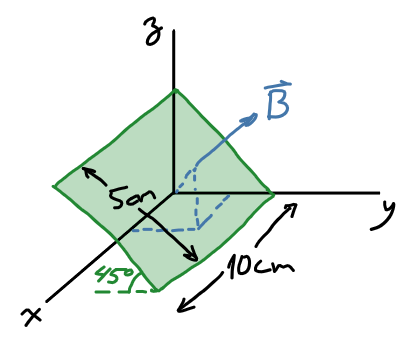
\includegraphics[width=4cm]{10-induction-electromagnetique/figures/flux-boucle-1.png}
    \end{center}
  }
  La boucle ci-contre est dans une région où se trouve un champ magnétique
  uniforme $\vB = \left(\vecxyz{1}{1}{1}\right) \si{G}$. Quel est le flux
  magnétique à travers la boucle?
\end{diapobox}

\begin{reponsebox}
  Le vecteur surface est $\vec{A} = \frac{ab}{\sqrt{2}}(\yhat + \zhat)$. Le
  flux est donc
  \begin{align*}
    \Phi_B &= \vB \cdot \vec{A}  \\
           &= \frac{ab}{\sqrt{2}}  (1 + 1) \si{G}  \\
           &= 5 \sqrt{2} \times 10^{-7} \si{\weber}
  \end{align*}
\end{reponsebox}




\section{Loi de Faraday}

\marginnote{
  Lafrance \S 10.3, 10.4
}

Une observation que vous avez faite au laboratoire est qu'un champ magnétique
variable induit une f.é.m. dans une boucle de fil conducteur. Faraday a
découvert que la f.é.m. induite est proportionnelle au taux de variation du
flux magnétique.
\begin{fondamentalbox}
  \minisec{Loi de Faraday}
  $$\emf = -\frac{d\Phi_B}{dt}$$
\end{fondamentalbox}
Le signe positif de la fém correspond à la direction des doigts de la main
droite lorsque le pouce est dans la direction du champ magnétique externe.

Dans le cas d'un champ uniforme et d'une boucle plate, on a
\begin{align*}
  \frac{d\Phi_B}{dt} &= \frac{d}{dt} \vB \cdot \vec{A} \\
                     &= \frac{dB}{dt} A\cos\theta + B \frac{dA}{dt} \cos\theta
                     + BA \frac{d\cos\theta}{dt} \\
                     &= \frac{dB}{dt} A\cos\theta + B \frac{dA}{dt} \cos\theta
                     - BA \sin\theta \frac{d\theta}{dt}
\end{align*}
Donc on peut obtenir une fém induite en faisant varier soit la grandeur du
champ, soit l'aire, soit l'orientation de la boucle dans l'espace.

Le courant dans la boucle peut circuler dans deux directions différentes. Pour
déterminer la direction, on utilise la loi de Lenz:

\begin{fondamentalbox}
  \minisec{Loi de Lenz}
  Le courant induit dans la boucle circule de façon à générer un champ
  magnétique induit qui s'oppose à la variation de flux magnétique.
\end{fondamentalbox}


\begin{diapobox}
  \minisec{Exemple d'application de la loi de Lenz}

  \marginnote{
    \begin{center}
      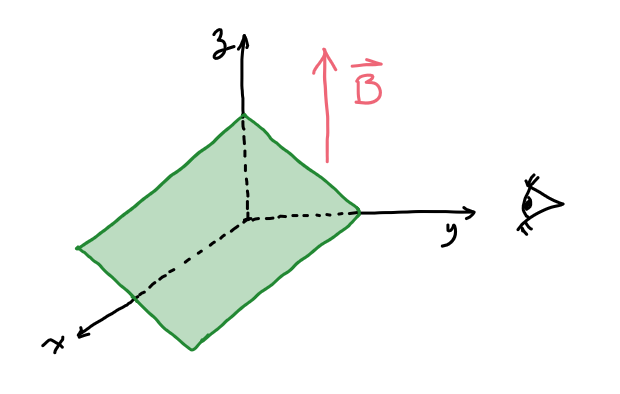
\includegraphics[width=4cm]{10-induction-electromagnetique/figures/boucle_oeil.png}
    \end{center}

    \begin{center}
      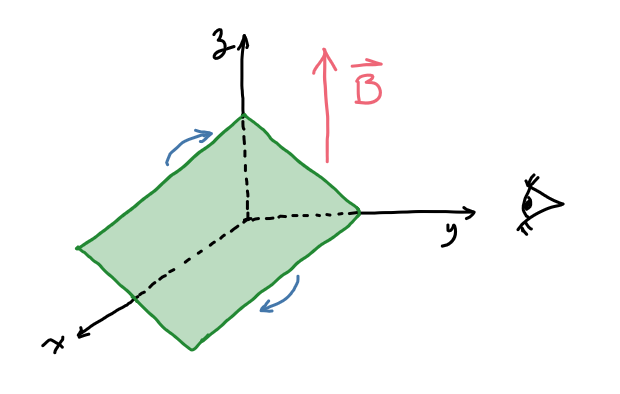
\includegraphics[width=4cm]{10-induction-electromagnetique/figures/boucle_oeil_tourne.png}
    \end{center}
  }

  Une boucle de fil se trouve dans un champ magnétique uniforme tel qu'illustré
  sur le dessin ci-dessous.

  La grandeur du champ magnétique augmente avec le temps. Quelle est la
  direction du courant induit dans la boucle?

  La grandeur du champ magnétique diminue avec le temps. Quelle est la
  direction du courant induit dans la boucle?

  La boucle tourne dans le sens indiqué sur le dessin. Quelle est la direction
  du courant induit dans la boucle?

  \begin{enumerate}
    \item sens horaire
    \item sens anti-horaire
    \item aucun courant induit
  \end{enumerate}

\end{diapobox}


\begin{diapobox}
  \minisec{Loi de Faraday - Champ magnétique variable}
  \marginnote{
    \begin{center}
      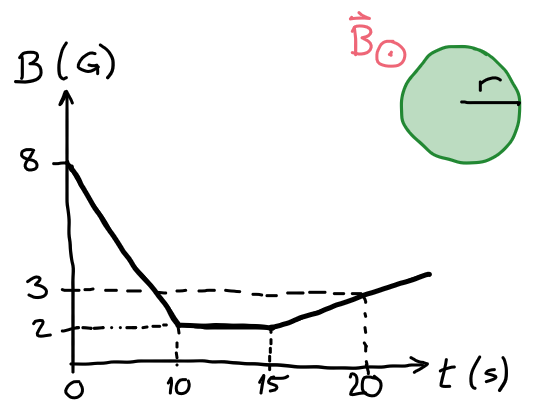
\includegraphics[width=4cm]{10-induction-electromagnetique/figures/champ_variable.png}
    \end{center}
  }
  Une bobine circulaire de \SI{5}{\centi\meter} de rayon comportant \num{50}
  tours se trouve dans un champ magnétique uniforme dont la grandeur varie dans
  le temps tel qu'illustré dans le graphique ci-dessous.

  Déterminez la f.é.m. induite et la direction du courant à
  \begin{enumerate}
    \item $t = \SI{5}{\second}$
    \item $t = \SI{11}{\second}$
    \item $t = \SI{20}{\second}$
  \end{enumerate}
\end{diapobox}

\begin{reponsebox}
  Le flux est
  \begin{align*}
    \Phi_B = \pi r^2 B N
  \end{align*}
  car le champ magnétique et le vecteur normal à la boucle sont dans la même
  direction. La f.é.m. est donc
  \begin{align*}
    \emf &= -\frac{d \Phi_B}{dt}  \\
         &= -\pi r^2 N \frac{dB}{dt}
  \end{align*}
  Puisque la grandeur du champ magnétique est linéaire par morceau, le taux de
  variation est simplement la pente du segment de droite approprié. On a donc
  \begin{align*}
    \emf_5 &= -\pi r^2 N \frac{\SI{2}{G} - \SI{8}{G}}{\SI{10}{\second} -
              \SI{0}{\second}}  \\
           &= \SI{0.2356}{\volt}
  \end{align*}
  Puisque le champ magnétique diminue, le flux diminue et le champ induit doit
  être dans la même direction que le champ externe et le courant est donc dans
  le sens anti-horaire par la RMD.


  À $t = \SI{11}{\second}$, le champ magnétique ne varie pas, donc il n'y a pas
  de f.é.m. induite.

  Enfin,
  \begin{align*}
    \emf_{20} &= -\pi r^2 N \frac{\SI{3}{G} - \SI{2}{G}}{\SI{20}{\second} -
              \SI{15}{\second}}  \\
           &= \SI{-0.07854}{\volt}
  \end{align*}
  Puisque le champ magnétique externe augmente, le flux augmente et le champ
  induit doit être dans la direction opposée au champ externe. Le courant est
  donc dans le sens horaire par la RMD. 

\end{reponsebox}



\begin{diapobox}
  \minisec{Générateur linéaire}

  Un cadre métallique fixe sert de support à une tige métallique mobile. La tige
  se déplace vers la droite à \SI{20}{cm/s} et sa longueur est de \SI{35}{cm}. Le
  champ magnétique externe est uniforme de \SI{120}{G}.
  Si la résistance de la boucle est de \SI{4}{\ohm}, déterminer le courant induit
  dans la boucle.

  \begin{center}
  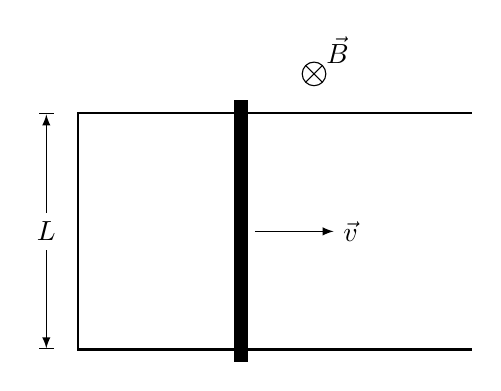
\begin{tikzpicture}[>=latex]
    \draw[thick] (5, 0) -- (0, 0) -- (0, 3) -- (5, 3);
    \draw[thick, fill] (2, -0.15) rectangle (2.15, 3.15);
    \draw[->] (2.25, 1.5) -- ++(1, 0) node[right] {$\vec{v}$};
    \draw[|<->|] (-0.4, 0) -- node[fill=white] {$L$} (-0.4, 3);
    \draw (3, 3.5) circle (0.15);
    \draw (2.894, 3.394) -- (3.1061, 3.6061);
    \draw (2.894, 3.6061) -- (3.1061, 3.394);
    \node at (3.3, 3.8) {$\vec{B}$};
  \end{tikzpicture}
  \end{center}
\end{diapobox}

\begin{reponsebox}
Le flux magnétique dans la boucle change parce que l'aire change. Dans un
intervalle de temps $dt$, l'aire change de
$$dA = Lvdt.$$
Autrement dit
$$\frac{dA}{dt} = Lv$$
Le flux magnétique est
\begin{align*}
  \abs{\Phi_B} &= BA
\end{align*}
donc le changement de flux est 
\begin{align*}
  \abs{\frac{d\Phi_B}{dt}} &= B \frac{dA}{dt} \\
      &= BLv
\end{align*}
Par conséquent
\begin{align*}
  \emf &= BLv \\
  I &= \frac{BLv}{R} \\
    &= \SI{0.2}{mA}
\end{align*}
Puisque l'aire augmente, le flux augmente donc la fém induite doit produire un
champ magnétique dans la direction opposée à celle du champ externe. Le courant
circule donc dans le sens anti-horaire.
\end{reponsebox}


\minisec{Générateur}

Une boucle rectangulaire tourne à vitesse angulaire $\omega$ dans un champ
magnétique externe $\vB$. Un courant alternatif sera produit dans la boucle.
La position angulaire de la boucle est donnée par
\begin{align*}
  \theta = \theta_0 + \omega t
\end{align*}
Le flux magnétique est
\begin{align*}
  \Phi_B = BA \cos(\theta_0 + \omega t)
\end{align*}
donc
\begin{align*}
  \emf = -\frac{d\Phi_B}{dt} = BA\omega \sin(\theta_0 + \omega t)
\end{align*}

Quelle est la tension efficace?

\begin{align*}
  \emf_\mathrm{eff} &= \frac{\emf_m}{\sqrt{2}} \\
                    &= \frac{BA\omega}{\sqrt{2}} 
\end{align*}

